\begin{ledgroupsized}[r]{120mm}
\footnotesize 
\pstart 
\noindent\textbf{\"{U}berlieferung:}
\pend
\end{ledgroupsized}
\begin{ledgroupsized}[r]{114mm}
\footnotesize 
\pstart \parindent -6mm
\makebox[6mm][l]{\textit{LiH}}%
Anstreichungen und Anmerkungen in \textsc{J. de Beaugrand},\protect\index{Namensregister}{\textso{Beaugrand,} Jean de 1595-1640}\cite{00334} \textit{Geostatice seu de vario pondere gravium secundum varia a terrae centro intervalla dissertatio mathematica}, Paris 1636: \textsc{Hannover}, GWLB,
Nm-A 10003. Der Band enth\"{a}lt weitere Marginalien, die nicht von Leibniz stammen.\pend
\end{ledgroupsized}
%\normalsize

\vspace*{5mm}
\begin{ledgroup}
\footnotesize 
\pstart
\noindent\footnotesize{\textbf{Datierungsgr\"{u}nde:}
Hinweise auf Beaugrands \textit{Geostatice} sind in den Stücken N.~10
%= LH37,5 Bl. 215 = De vitandis erroribus geometricis in re mechanica
und N.~11
%= LH35,8,30 Bl. 151 = Geometria amoenior
anzutreffen, welche beide von Leibniz datiert sind: N.~10 auf Dezember 1674; N.~11 auf April 1675.
Mutmaßlich wurden Leibniz' Marginalien in dieser Zeitspanne verfasst.
Eine frühere oder spätere Datierung ist jedoch nicht ausgeschlossen.}
\pend
\end{ledgroup}
\count\Afootins=1200
\vspace*{8mm}
\pstart 
\normalsize
\noindent[p. 4] \edtext{Ex schematis hic adiectis patet huius Theorematis\protect\index{Sachverzeichnis}{theorema} duodecim esse casus, quorum duo a Ptolemaeo Mathematicae constructionis libro primo capite vndecimo  [...]}{\lemma{}\Afootnote{\textit{Oberhalb dieses Textes zwölf Abbildungen, unter denen die hier aufgeführte} [\textit{Fig.~1}]. \textit{Daneben auf H\"{o}he der Linie ABGC notiert Leibniz:} $\displaystyle\frac{AC}{BC} \sqcap \displaystyle\frac{AD \frown EF}{DE \frown BF}$}}
\pend
\vspace{1.5em}
\begin{center}
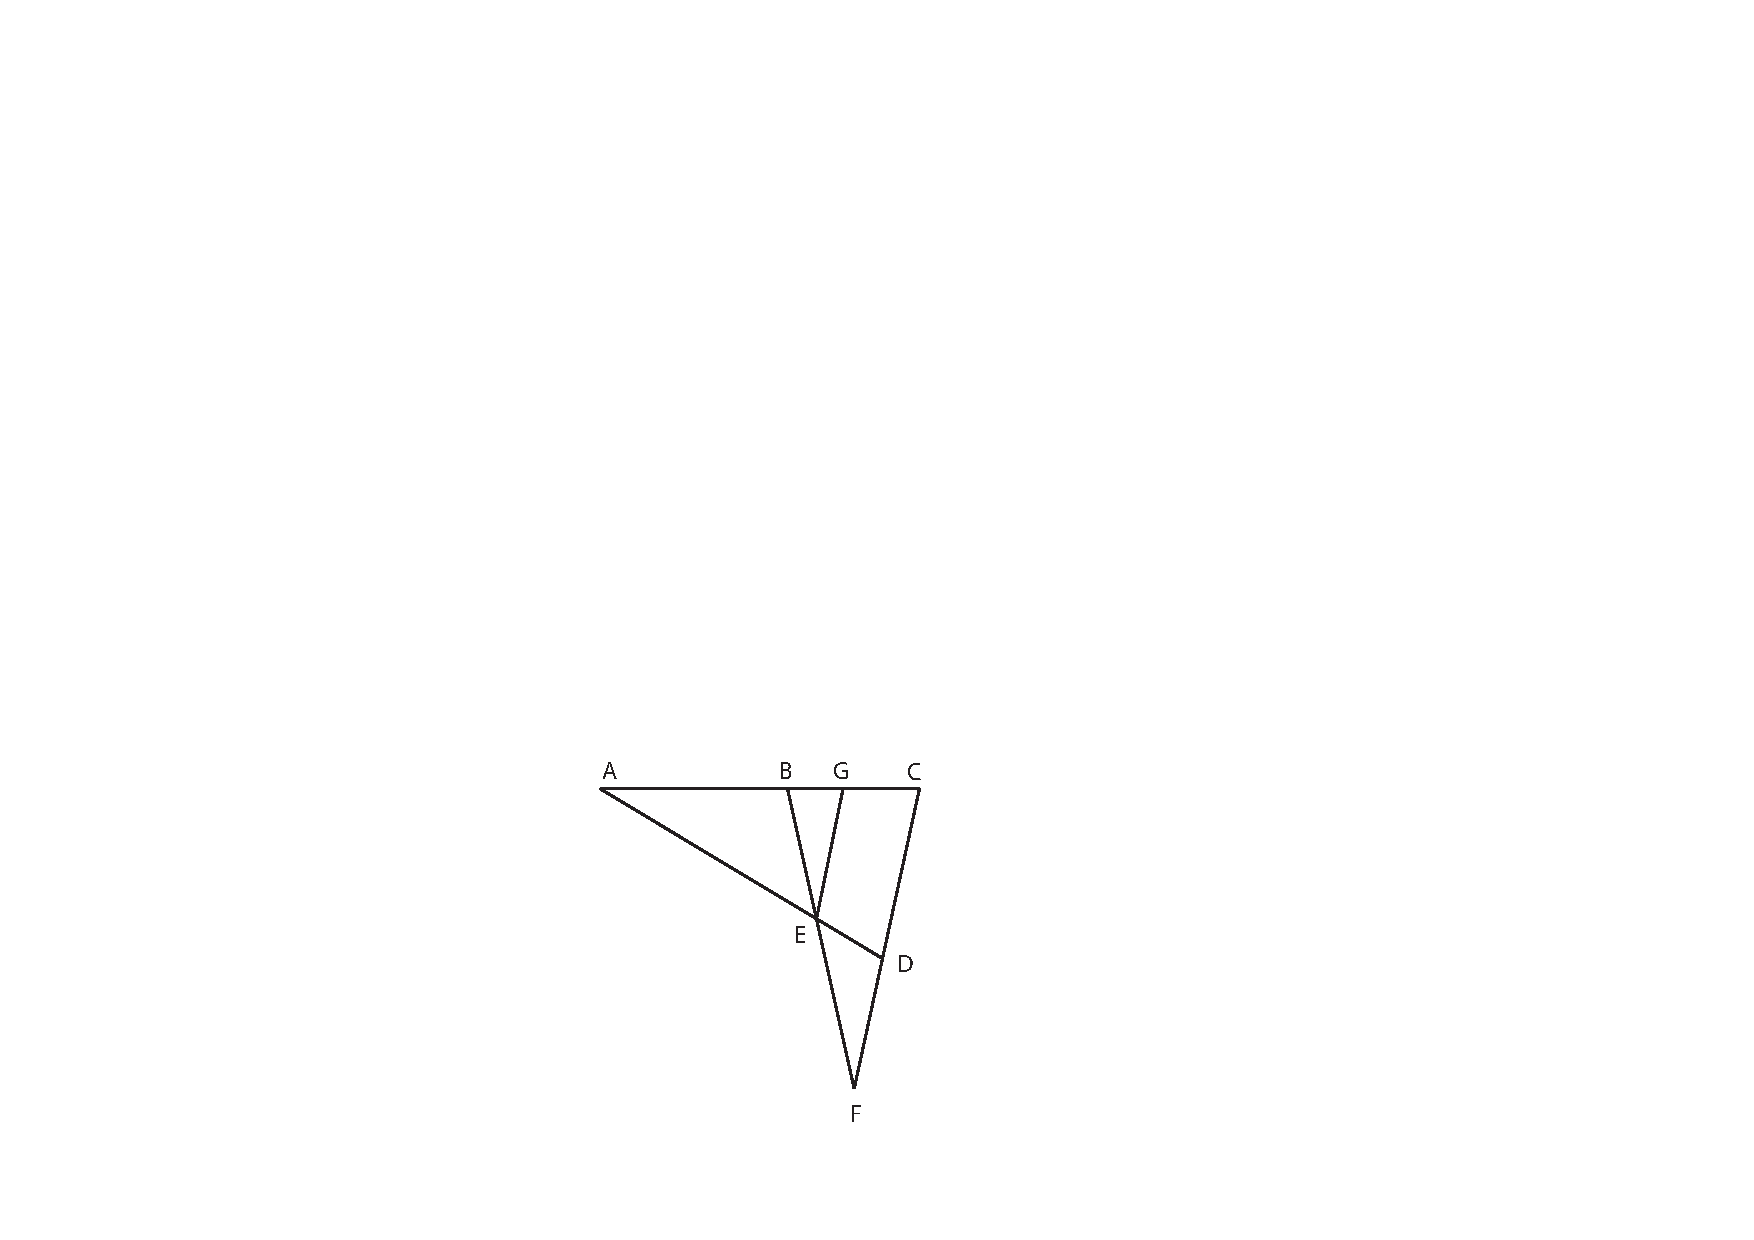
\includegraphics[width=0.4\textwidth]{images/beaugrand1636-d1.pdf}\\
 \noindent \centering [\textit{Fig. 1}]
\end{center} 
\newpage
\pstart  [p. 5] Siquidem ex praecedenti propositione ratio rectae $AB$ ad [p. 6] 
\edtext{rectam $BC$ composita est ex rationibus rectae $AE$ ad rectam $DE$ et rectae $DF$ ad rectam $FC$.}{\lemma{}\Afootnote{\textit{Oberhalb des Textes auf S. 6 vier Abbildungen, unter denen die hier aufgeführten} [\textit{Fig. 2}]. \textit{und} [\textit{Fig. 3}]. \protect\rule[-4mm]{0mm}{10mm}\textit{Dazwischen notiert Leibniz}: $\displaystyle\frac{AE}{ED} \sqcap \displaystyle\frac{CF}{DF}$, $AB \sqcap BC$, \textit{und} $\displaystyle\frac{AB}{BC} \sqcap \displaystyle\frac{AE}{DE} \frown \displaystyle\frac{DF}{FC}$.\vspace{1.8mm}}}
\pend
\vspace{2.5em} 
\pstart
\count\Afootins=1200
\begin{center}
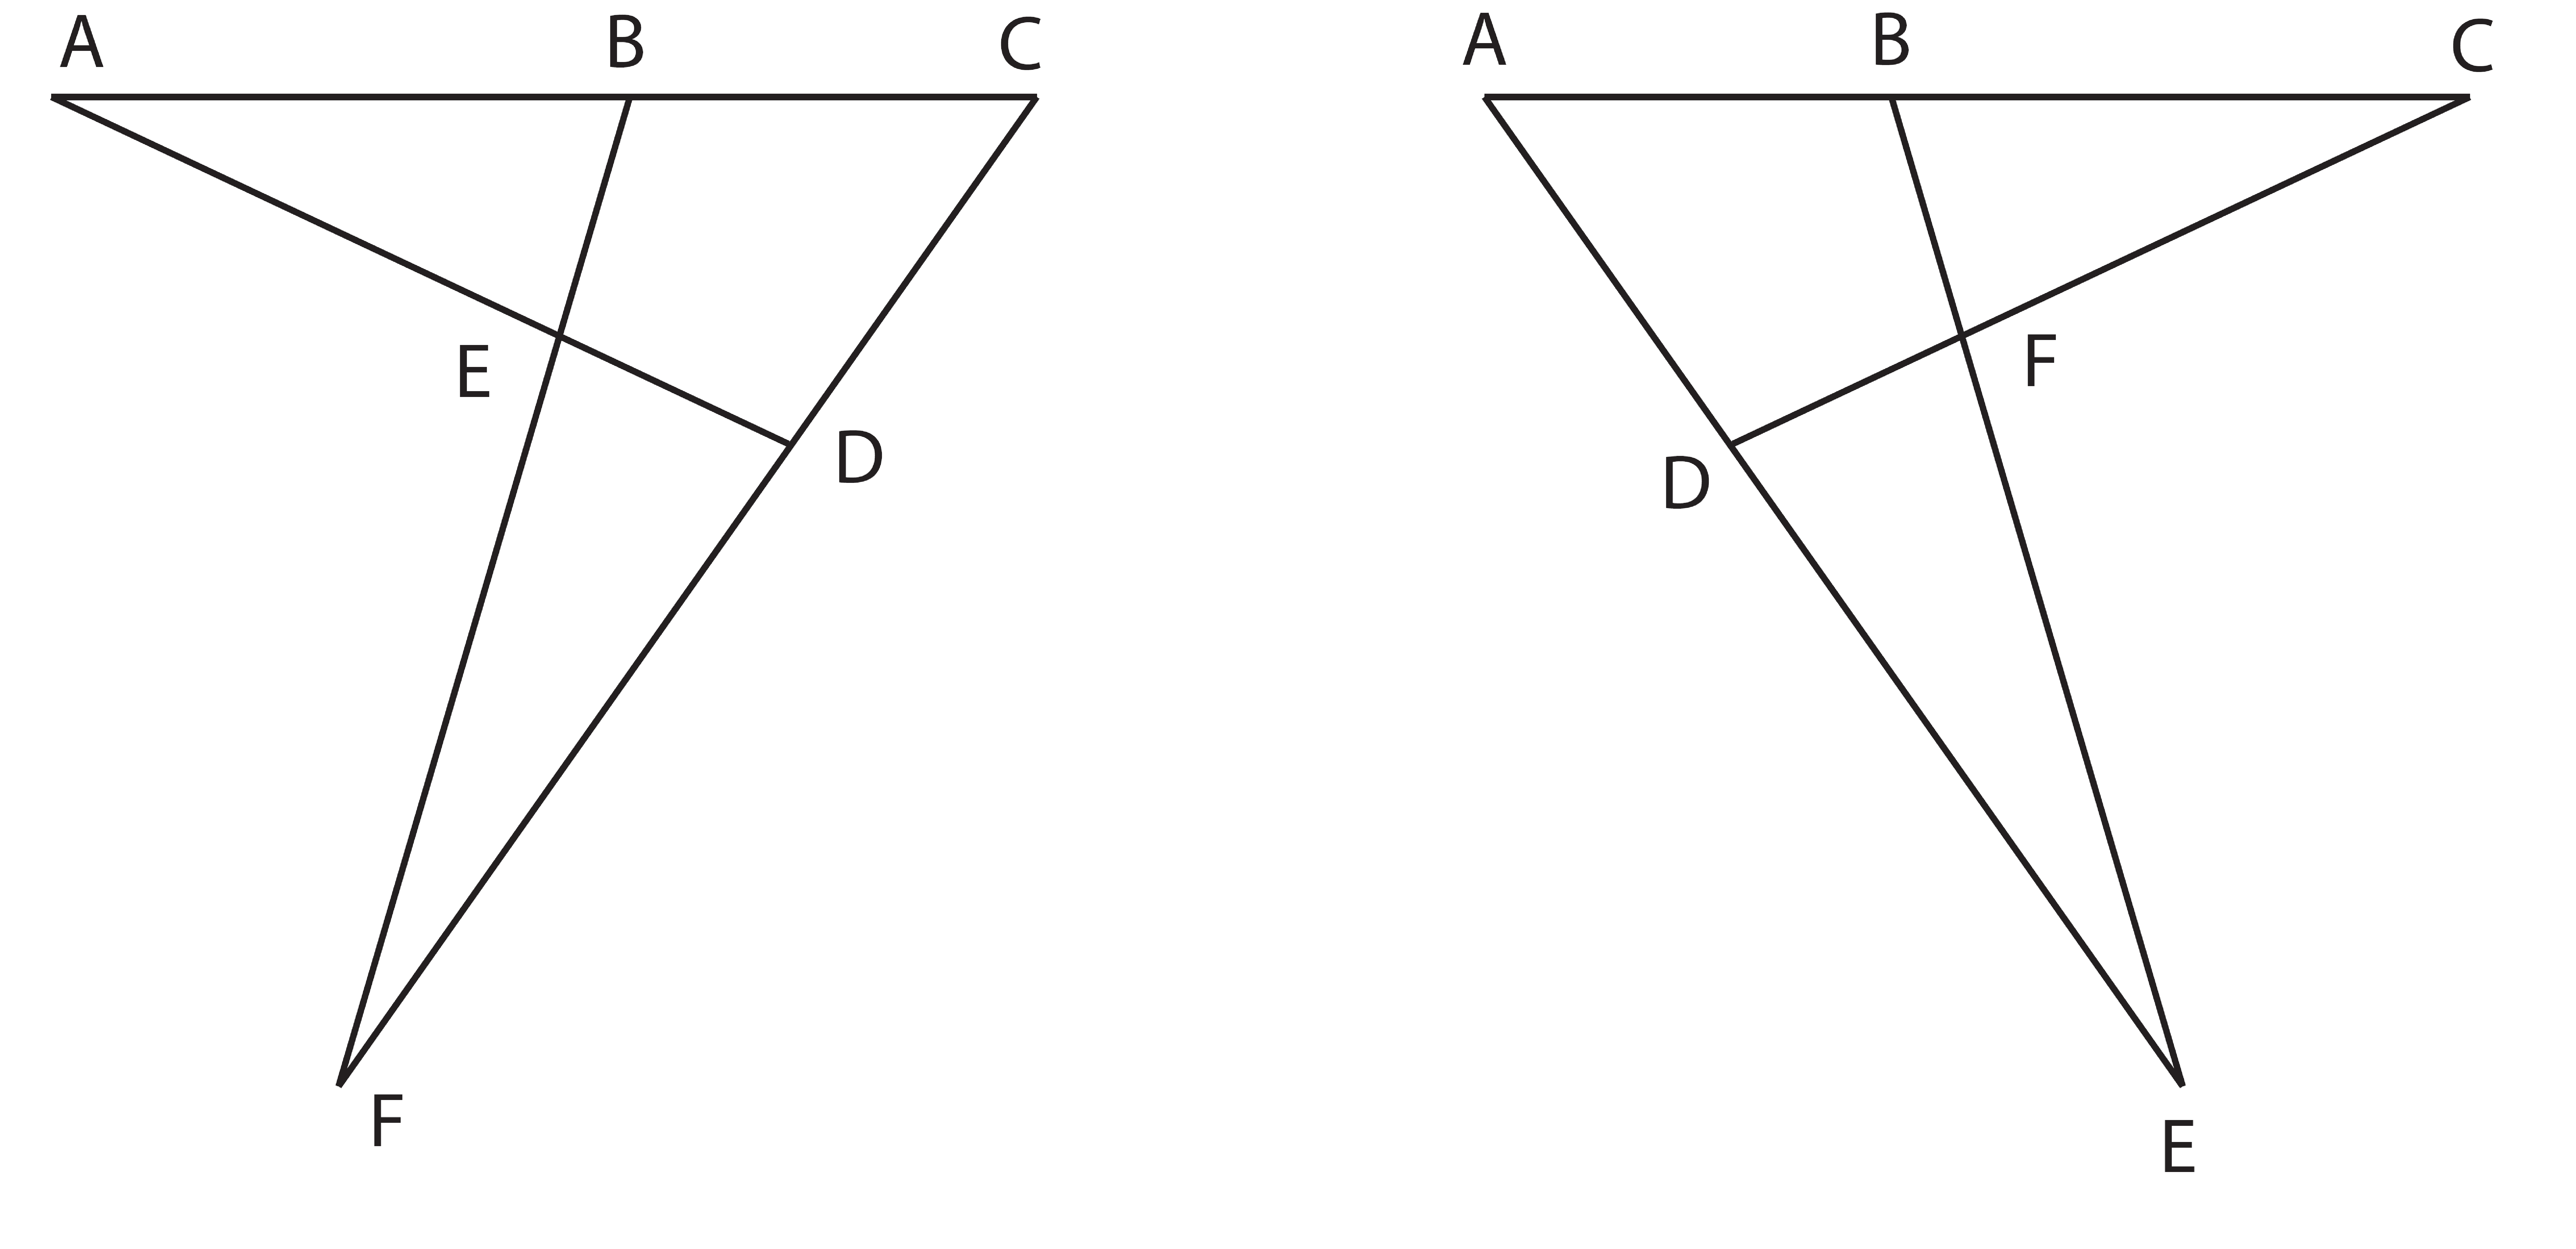
\includegraphics[width=0.9\textwidth]{images/beaugrand1636-d3.pdf}
\end{center}
\hspace{25mm} [\textit{Fig. 2}]  \hspace{58mm}   \lbrack\textit{Fig. 3}\rbrack
\pend
\vspace{2em} 
\pstart [p. 8] \setline{3}Quare \edtext{cum punctum $H$ diuidat rectam $FE$ quae conjungit}{\lemma{}\Afootnote{\textit{Oberhalb dieses Absatzes, gestrichen}: Quaestio est, an hoc Archimedis principium verum sit, cum linea non est parallela horizonti, hoc demonstrandum.\vspace{1.8mm}}}\edtext{}{\lemma{Archimedis principium}\Cfootnote{\textit{De planorum aequilibriis} I,6.}} centra grauium \textit{I, B} in proportione reciproca suorum ponderum\protect\index{Sachverzeichnis}{pondus}, centrum grauitatis\protect\index{Sachverzeichnis}{centrum gravitatis} vtriusque simul erit in puncto $H$, vti ab Archimede primo Aequiponderantium libro et a nobis in Mechanicis noua methodo demonstratur.
\pend 
\newpage
\pstart  [p. 8] Sed ex constructione punctum $H$ est in recta puncta \textit{A, G} [p. 9] conjungente, quare si concipiatur rectam $FD$ esse libram \edtext{cuius centrum sit in puncto $G$}{\lemma{}\Afootnote{\hspace{1.8mm}\textit{Leibniz unterstreicht doppelt}: cuius centrum sit in puncto $G$, \textit{und notiert dar\"{u}ber}: hoc probandum}}, rectae \textit{FG, GD} brachia [...]
\pend 
\pstart  [p. 9] Igitur si a puncto $G$ libra $FD$ suspendatur, grauium $I$ in $F$ et $B$ in $E$ librata ponderibus immobilis haerebit, hoc est, pondus grauis $I$ in $F$ aequabitur ponderi grauis $B$ in $E$.\edtext{}{\lemma{}\Afootnote{\hspace{1.8mm}\textit{Am Ende des Absatzes, gestrichen}: hoc impossibile, si recta $A$}}
\pend 
\pstart  [p. 11] \edtext{Enimuero, postulante Archimede\protect\index{Namensregister}{\textso{Archimedes}, 287-212 v. Chr.}, grauia aequalia ex distantijs aequalibus aequeponderant}{\lemma{}\Afootnote{\hspace{1mm}\textit{Am Rand}: Ita scil. si lineae directionis parallelae.}}. Dicet forsitan aliquis Archimedem in Aequeponderantium libris lineas directionis grauium utpote $AC, AB$ sibi mutuo parallelas supposuisse, non secus atque in libro de Quadratura Paraboles\protect\index{Sachverzeichnis}{parabola}.\pend \pstart [p. 23] Rationes datae \edtext{sunto \textit{A} ad \textit{B} et \textit{C} ad \textit{D}}{\lemma{}\Afootnote{\textit{Oberhalb A}: $\displaystyle\frac{A}{B}$\  $\displaystyle\frac{4}{5}$. \textit{Oberhalb C}: $\displaystyle\frac{C}{D}$\  $\displaystyle\frac{8}{10}$.}} quae simul sint componendae. Ducatur $A$ in\edtext{}{\lemma{}\Afootnote{\textit{Oberhalb} in \textit{zwischen A und C}: $AC$}} $C$ et $B$ in\edtext{}{\lemma{}\Afootnote{\textit{Rechts oberhalb B}: $BD$}} $D$ sintque producti \textit{E,G}\edtext{}{\lemma{}\Afootnote{\textit{Oberhalb} $E$: $AC$, \textit{oberhalb} $G$: $BD$}}. Dico rationem $E$ ad $G$ componi ex rationibus $A$ ad $B$ et $C$ ad $D$.
\pend
\count\Afootins=1500
 


 


 


 

